% -*- coding: utf-8 -*-

\documentclass{article}
\usepackage{subfig}
\usepackage{listings}
\usepackage{graphicx}
\usepackage{amsmath}
\usepackage{amssymb}
\usepackage{amsthm}
\usepackage{algorithm2e}
\usepackage{booktabs}
\usepackage{enumerate}
\usepackage{longtable}
\usepackage{caption}
\usepackage{verbatim}
\usepackage[colorlinks=true]{hyperref}
\usepackage[top=1in, bottom=1in, left=1.5in, right=1.5in]{geometry}


% THEOREMS -------------------------------------------------------
\newtheorem{thm}{Theorem}[section]
\newtheorem{cor}[thm]{Corollary}
\newtheorem{lem}[thm]{Lemma}
\newtheorem{prop}[thm]{Proposition}
\newtheorem{prob}{Problem}
\theoremstyle{definition}
\newtheorem{defn}[thm]{Definition}
\newtheorem*{sol}{Solution}
\theoremstyle{remark}
\newtheorem{rem}[thm]{Remark}
\numberwithin{equation}{section}
% MATH -----------------------------------------------------------
\newcommand{\norm}[1]{\left\Vert#1\right\Vert}
\newcommand{\abs}[1]{\left\vert#1\right\vert}
\newcommand{\set}[1]{\left\{#1\right\}}
\newcommand{\tuple}[1]{\left \langle #1\right \rangle}
\newcommand{\Real}{\mathbb R}
\newcommand{\eps}{\varepsilon}
\newcommand{\To}{\longrightarrow}
\newcommand{\BX}{\mathbf{B}(X)}
\newcommand{\A}{\mathcal{A}}
% ----------------------------------------------------------------

\begin{document}
\bibliographystyle{plain}
\title{SuperGo: The Manual}
\author{Linpeng Tang, Qin Liu, Jiayuan Ma, Jiajun Shen}

\maketitle

\begin{abstract}
%by Mark Mar
This report is an introduction to our artificial intelligence course project SuperGo, a Monte-Carlo method based computer Go agent. In this document, we briefly summarize main techniques in devising a computer Go agent, including Monte-Carlo method, heuristic evaluation, domain knowledge, opening book and pattern matching.
\end{abstract}

% -*- coding: utf-8 -*-


\section{Monte-Carlo Method}
As the search space of Go is too large (the game tree is in the order of $10^{360}$ for alpha-beta tree search \cite{bouzy2001computer}, one major alternative to using hand-coded knowledge and searches is the use of Monte-Carlo methods.

In the Monte-Carlo method, when we need to evaluate the current state of a Go board (say, we need to estimate whether Black is more likely to win than White), we simply simulate ``random'' plays on the board and see what happens when the simulation of the game ends. Alpha-beta tree search doesn't work well for computer Go, because on the one hand it is impossible to search the whole tree until it reaches the terminal state, and on the other hand if we only search for several steps the evaluation may be very inaccurate. In Go a good move may not seen to be useful until many steps later. The Monte-Carlo method, however, overcomes this difficulty because it simulates to the end of the game, when the state can be easily evaluated.

The Monte-Carlo method also has the advantage that it requires little hand-coded domain knowledge, and is easy to code. Compared to pattern matching, it also can make good use of the increasing power of modern computers. Actually, it is showed that with the growth of simulation times, the win-rate of a Monte-Carlo based computer Go program against a traditional program grows accordingly\cite{enzenberger2010fuego}. And it is proven theoretically that when the number of simulations approaches infinity, Monte-Carlo methods will eventually give a accurate evaluation of the board (as the exhaustive alpha-beta tree search)\cite{kocsis2006bandit}.

\subsection{Monte-Carlo simulation}
It is said in \cite{chaslot_combiningexpert} that the design of a good Monte-Carlo simulator is a dark art. A good Monte-Carlo simulator should give an accurate evaluation of the current state of game as fast as possible. This often requires a large amount of simulations, so the simulator should be very fast (SuperGo can do about 7000 simulations in 8 seconds in one 2GHz core). The simulator should not be totally random, i.e. choose randomly from all the legal moves. Instead, we should think of the simulator as simulating what two simple-minded players will do in a game---they will capture stones when they can, save stones from being captured when they can, or do some simple pattern matching. Curiously, it is said in in \cite{chaslot_combiningexpert} that a complicated simulator, even if given enough time, may not give a good result. For example, even if we use GNU Go as the simulator and simulate as many times as a simple simulator, the result of the evaluation may not be as accurate as the simple simulator. This is a curious property. It shows that the simulator must seek a balance between exploration and exploitation, between simplicity (randomness) and sophistication. SuperGo's simulator largely borrows the methods of Fuego\cite{grace2010fuego}, employing some greedy heuristics (like Nakade, Atari capture and Atari defense) and local pattern matching.

\subsection{Upper Confidence Tree Search}
UCT (Upper Confidence Tree) Search, originally proposed in \cite{kocsis2006bandit}, is a general framework for planning with Monte-Carlo simulations. It seeks a balance between exploration and exploitation. Consider the game tree in computer Go, every node typically has $80$ children for a $13\times 13$ board, and the game tree typically has a height of more than $100$. Now suppose we have searched some part of the tree, what should we do next? There are two options, the first is to pick the best result we have met so far and keep expanding the path (exploitation); the second is to pick a new path and start over (exploration). Note there are problems with both approaches: if we only focus on the best result we have achieved so far, we may be trapped in a local minimum and miss other good results, and if we spread our searches among all the paths, since there are so many paths, we can not expand each path deep enough and the evaluation may be inaccurate after all. UCT Search addresses this problem by combining the two approaches, it gives each node a UCT bound \cite{grace2010fuego}:
\begin{equation}
\text{UCT Bound} = x_j + c \sqrt {\frac {\log n} {T_j(n)}} = \text{Estimated Move Value + UCT Bias}
\end{equation}
\begin{itemize}
\item $x_j = \text{reward for move $j$} = \text{weighted mean of move value and RAVE value}$
\item $j   = \text{move index}$
\item $n   =  \# \text{times father node visited}$
\item $T_j(n)  =  \# \text{times move j has been played}$
\item $C    =  \text{appropriate constant (default is $0.7$ in Fuego)}$
\end{itemize}

And when expanding a path, we choose the child of a parent node with the largest of UCT bound.

Intuitively, the UCT bound consists of two parts, the Estimated Move Value represents the exploitation part, and the UCT Bias represents the exploration part. We will favor those nodes that has high estimated move values and has been visited few times compared to its parent.

\subsection{Rapid Action Value Estimation}
We need some heuristics to pick the most hopeful moves from the large number of possible moves of a given game state. RAVE (Rapid Action Value Estimation) \cite{gelly2011monte} provides a good way for doing that, using information generated in the Monte-Carlo simulation. The basic observation of RAVE is that is a move several steps later contributes to a win in the current state, then it may benefit us to play it now as well. Now given a sequence of simulated moves $x_0, x_1, \dots x_{2m-1}$, and suppose that $x_{2k}$ is played by Black and $x_{2k+1}$ is played by White. Suppose in this simulation Black wins. Then we will add some positive rating to those nodes of Black Moves that have the same moves with $x_0, x_2, \dots, x_{2m-2}$ (showing that these moves may be desirable), and add some negative rating to those nodes of White Moves that have the same moves with $x_1, x_3, \dots, x_{2m-1}$ (showing that these moves maybe undesirable). Further more, the larger $i$ is, the less impact $x_i$ will have on the corresponding nodes.


\subsection{The UCT Search Framework}
Now we are ready to state the UCT Search framework for computer Go. We wish to expand the whole game tree in the memory, with the current state being the root node of the tree. But as this is impossible for Go, we only store some nodes near to the root in memory, and store four values in each node: visit-count, visit-rating, rave-count, rave-rating.
\begin{itemize}
  \item visit-count: how many times this node has been visited in a simulation path.
  \item visit-rating: the win-rate of the Black player of all simulations visiting this node.
  \item rave-count: the weight of the RAVE heuristics.
  \item rave-rating: the value of the RAVE heuristics.
\end{itemize}

Every time we we start a search from the root of the tree, and the search consists of two phases: in-tree phase and play-out phase. During the in-tree phase, we select child of the current node by the heuristics of UCT and RAVE combined (note that however in every step the corresponding player will choose a move that benefits him best and does most damage to his opponent). When we reach a terminal node of the tree, we check whether this node represents the end of a game. If it does, we directly update the four parameters above of the nodes in the tree. Otherwise, we start a simulation, evaluate the result of the simulation and then update the statistics.

\begin{figure}
  \centering
  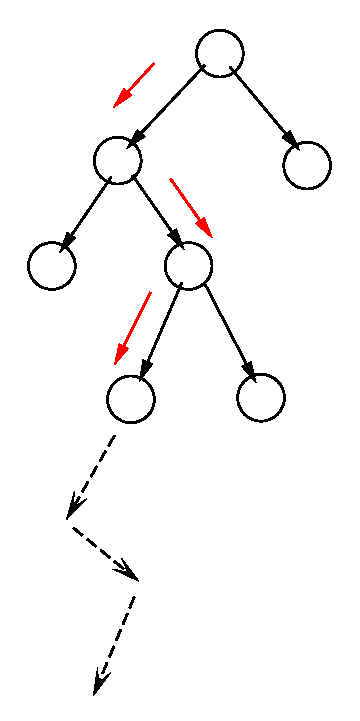
\includegraphics[width=.2\textwidth]{tree.eps}\\
  \caption{A sample game tree in during a UCT search. The red dashed arrow-headed lines represents a search path, including a in-tree part and a play-out simulation part}\label{fig:tree}
\end{figure}

\subsection{Engineering and Some Innovations}

\subsubsection{Parallel Search Infrastructure}
In SuperGo we implemented a simple UCT Search Go framework, equipped with RAVE heuristics a greedy simulator. As more simulations usually results in a more accurate evaluation, SuperGo supports multi-threaded simulations. As the game-tree is a public resource, it should be protected with a lock. \cite{enzenberger2010fuego} also proposes a lock-free infrastructure that can improve the number of simulations at the cost of some minor inconsistencies, and that structure was employed in Fuego. In our experiments, SuperGo can do about $7000$ simulations in one core. And with two threads running one two cores, we can double the number.

\subsubsection{Combining UCT Simulations with Expert Knowledge}
With our observation, UCT search with Monte-Carlo simulation results in a AI player with great overall understanding of the board, but is usually weak in some local, strategic moves. To compensate this, we add expert knowledge with the statistics generated by UCT search when we generate our next move for the game. Originally, after many times of simulation, the AI will select the move corresponding to the child of the tree root with the highest visit-value. Now we multiply visit-value by an additional coefficient, representing how the expert knowledge. For example, we may give a capture move a $1.5$ coefficient, and give a cut move a $1.2$ coefficient.

\subsubsection{Different Strategies for End Game Phase}
Monte-Carlo simulation can be quite weak in the open game phase and end game phase. In the open game phase, the visit-rating and visit-count of most moves are similar, because after so many steps to the end of the game, the influence of the moves at the open game is too small to be detect by the Monte-Carlo simulator. In the end game phase, since the the win/loss state is already determined, the simulator often gives a win-rate of of near 1 (indicating that Black is very likely to win) or near 0 (indicating that White is very likely to win). So this would give little hit about what move should be executed next. To cope with this problem, in the end game phase (when there are less than 60 possible moves for a player), we give more weight to those wins with a better results (wins more area). This improvement will make SuperGo more rational at the end of the game, like trying to occupy more area at the boundary.

\subsubsection{Dynamic Komi}
With our observation, the Monte-Carlo method suffers from the problem of being weak then it is in large advantage of in large disadvantage. Because in either of these two situations, the win-rate of every moves will be very similar no matter what move the AI plays. To cope with this problem, we can give those results with large win (loss) higher reward (punishment). This approach, however, is theoretically unsound, and doesn't give good results in experiments. We take a different approach by changing the Komi dynamically. That is, we record the most recent $K$ (say $K=8000$) evaluations and update the Komi with the median of the recent evaluation results after every $K$ simulations. In this way, the win-rate of the simulations will vary around $0.5$ no matter whether the AI is in advantage or disadvantage, and the Monte-Carlo simulations can always give us valuable information about what is the best move next.

In our experiment, this technique seems to make SuperGo more reliable, and can greatly improvement its performance against our competitors.


% territory reward

% bias, atari, connect

% dynamic ko

% ----------------------------------------------------------------

%nakade
%influence
%eye
%unconditional life
%chain
%region
%board

\section{Improving Monte-Carlo Simulations}

As introduced in the last section, we need to use the result of Monte-Carlo (MC) simulations to evaluate the probability of winning of current state in the MC tree search. In this section, we combine some expert knowledge to help us better estimate the probability.

\subsection{Efficient board representation}

In order to run more MC simulations in limited time, we need more efficient board representation. The class \emph{GoBoard} defines a Go board that implements the rules of Go and provides a lot of helper functions to get blocks, liberties, adjacent blocks, and so on. We use a 1-D array to represent the board which is faster than the normal 2-D representation. To accelerate the operations of play a move, we need to maintain a data structure that stores the information of blocks in the current board and their liberties.

The class \emph{GoUctBoard} is optimized for Monte-Carlo simulations. In contrast to class \emph{GoBoard}, this board makes certain assumptions that are usually true for Monte Carlo simulations for better efficiency:
\begin{itemize}
  \item No undo
  \item Alternating play
  \item Simple-Ko rule
  \item Suicide not allowed
\end{itemize}

\subsection{The `Nakade' Problem}

Nakade refers to a situation in which a group has a single large internal, enclosed space that can be made into two eyes by the right move --- or prevented from doing so by an enemy move. When the group is dead, the MC simulator which plays random moves sometimes estimates that it lives with a high probability. Therefore, the tree will not grow in the direction of right move. 

This will lead to a false estimate of the probability of winning. To reflect the effect of a nakade, we use the below algorithm\cite{chaslot_combiningexpert}: if a contiguous set of exactly 3 free locations is surrounded by stones from the opponent, then we play at the center (the vital point) of this ``hole''.

\subsection{Unconditional Live}

A set of chains of a player is said to be pass-alive if none of the chains in this set can be captured even if the player always passes. However, the above definition can be tedious to apply, because the required search space to prove pass-alive can be large. Benson \cite{benson1976life} defined the concept of unconditional life in a way that is easier to apply, because no search is required. At the same time, Benson also proved that a set of chains is unconditionally alive if and only if it is pass-alive. As such, unconditional life and pass-alive have become synonyms.

Benson's definition of unconditional life also leads to an algorithm for finding chains that are unconditionally alive, known as Benson's algorithm. This algorithm is not easy to apply manually, and therefore is intended for computer life-and-death programs.

With Benson's algorithm, when we find a set of chains is unconditional live, we can concentrate on other areas on the board which can reduce meaningless moves in MC simulations.  % by LQ
\section{Construction and Usage of Opening Books}

Games are usually divided into three phases: opening, middlegame and endgame. In any of the three phases, the default action of a computer program is to start a brute force search for a ``best'' move. Since such a search has to be performed within a limited time, it can only examine nodes down to a certain depth, which means that the calculated value is only a heuristic approximation of the game-theoretic value\cite{lincke2002openbook}.

Under such circumstances, strategies of using precalculated ``references'' have come into being. Such ``references'', in the parlance of games, are called books. Books designed for the opening phases of the game are called opening books, while books used in endgames are endgame books.


\subsection{Opening Books for Go}

An opening book is an important feature of any game-playing computer program. These books used to be constructed manually by an expert, by storing good moves suggested by theory, or simply by listing all games ever played by
strong players.

An opening book is especially useful in Go since Go has an extremely large search space in the opening phase of a game. Using a precalculated book will greatly improve the performance of a computer Go and save the time in a time-limited competition.

During the history of Go game, human players have generalized several systematic theories in the opening phase of Go game. Fuseki, a Chinese word coined to represent initial sequence of moves in a game, is famous among professional Go players. Only a proportion of fusekis have recognized or specific names. These include the two-star fuseki, three-star fuseki, Chinese fuseki, Kobayashi fuseki, and Shusaku fuseki.

Generally, there are two types of fusekis, both of which have their own theoretical background:
\begin{itemize}
\item \textbf{Territorial approach}
As played on a large board (the standard $19 \times 19$ Go board), the priority is given to playing corner enclosures, then to extending to the middle of the sides, and finally to the center because it is easier to secure territory in the corners than on the sides or in the center.
\item \textbf{Influence-oriented approach}
Unlike the territory-oriented playing style, this approach emphasizes control of the center. The reason for this is that one's play should not be narrowly focused on attempting to secure points quickly by occupying the corners first. Although it requires more effort to secure the center, it is more profitable since the center constitutes the majority of territory on the board.
\end{itemize}

\subsection{Opening Books in SuperGo}

In our SuperGo project, we adapt the opening book from Feugo. As the opening book of Feugo is largely for the $19 \times 19$ Go board, we have to process it in order to make it usable and reasonable in the $13 \times 13$ Go board. We use a mapping which maintains the locations of $9$ special points on the board. To be more specific, a rough mapping table is provided:

\begin{center}
\begin{tabular}{c|c}

19x19 & 13x13 \\ \hline
D4 & D4 \\
D10 & D7 \\
D16 & D10 \\
K4 & G4 \\
K10 & G7 \\
K16 & G10 \\
Q4 & K4 \\
Q10 & K7 \\
Q16 & K10 \\
\end{tabular}
\end{center}

The other points in the 19x19 line goban is randomly mapped into the 13x13 line goban according to the adjacent situations of the point on the board.

Since the board in the opening phase of the game contains very few stones, it is rather cumbersome to represent the whole board in the opening book\cite{lincke2002openbook}. Instead, we use a sequence of strings to represent a sequence of initial moves of a game. For example,
\begin{verbatim}
Q4 Q16 C4 D16 C14 F17 | D10
\end{verbatim}
represents the first six moves followed by a next move D10 suggested by the book. This representation is cheap to store and easy to match.
 % by Mark Mar
\section{Pattern Matching}

This part integrates some of knowledge of human Go players into SuperGo. We have stored some existed patterns (or Joseki) in our SuperGo to make it ``think'' more like a human player. 

When several candidate moves have been generated by Monte-Carlo simulation, each move is then matched to see if it follows a Joseki stored in our pattern database. If a candidate move matches a Joseki quite perfectly, it is highly likely that this is a quite good move. Therefore, a candidate move that matches a Joseki is given higher score so that a move generator will have a higher possibility to choose it.

Compared with Monte-Carlo simulation, pattern matching is more rigid and yields high efficiency. Actually, using pattern matching techniques in Go game is similar to ``standing on the giants' shoulders''.

\subsection{Pattern Representation}

Most of the patterns we use in SuperGo only consider the local situations. Hence, we use a standard way to represent these patterns. We use two-dimensional char arrays to store local patterns. The examples are as follows:

\begin{verbatim}
                               ?.??           ??xx?
                               O*.O           O.xx?
                               .X..           .?X.O
                                              .O*..
                                              .....
                                              -----
\end{verbatim}

The different symbols stand for different meanings, and they are shown as follows. Such representations are easy for the human to read and comprehend.

\begin{center}
\begin{tabular}{l|l}
\textbf{Symbols} & \textbf{Meanings} \\ \hline
$?$ & don't care \\
$.$ & empty \\
$X$ & your stone \\
$O$ & your opponent's stone \\
$x$ & your stone or empty \\
$o$ & your opponent's stone or empty \\
$*$ & your next recommended move \\
$-$ or $\mid$ & edges of board \\
$+$ & corner of board \\
\end{tabular}
\end{center}

\subsection{Matching and Scoring}

We have stored over $2000$ patterns in our pattern database. When doing matching, we have also taken into consideration rotations, reflections of patterns. Therefore, we have a combination of over $100000$ patterns in SuperGo.

Candidate moves that satisfy more patterns will receive a higher score, matching a corner pattern will earn a candidate move higher score, and matching a larger pattern (ie. $8 \times 8$ array) will be given higher ratings.
 % by Mark Mar
\section{Future Work}
SuperGo is able to beat most of its opponents in the small competition. But still a lot of work remains to be done. We think the following tips can improve SuperGo's performance or deserve further investigation.

\begin{itemize}
\item Dynamic Komi. According to our observation, dynamic Komi enhanced SuperGo's performance against its performance. And this technique is actually applicable to all MC algorithms--dynamically changing the criteria of winning/losing to make Monte-Carlo simulation provide more discriminating results. We plan to test this technique in Fuego and see how it works.

\item Pattern Matching. Compared to other advanced Go agents such as GNUGo, pattern matchings in SuperGo is far from accurate. In GNUGo, every pattern is annotated with additional information and constraints. Patterns in GNUGo are less rigid but can be used more appropriately by machines. 

The current problem of pattern matching in SuperGo is that moves generated by pattern matching tend to be densely located in a small region. This is not a optimum strategy in the opening phase of the game.
In future, more abundant and clever patterns will be implemented in SuperGo.

\item More Heuristics. Currently, SuperGo has not implemented all the heuristics. We may try to create more eyes, connect existing chains and prevent the opponents from connecting their chains.

\item Safety Solver. We may use more sophisticated algorithms like the unconditional life algorithm to prune the unnecessary moves in Monte-Carlo simulations. In this way we can make the simulations more efficient and provide more accurate predictions. 

\end{itemize}

\bibliography{library} % the references
\end{document}
% ----------------------------------------------------------------
